\documentclass[tikz]{standalone}
\usepackage{pgfplots}
\usepackage{xcolor}
\usepackage{booktabs}
\definecolor{brown}{HTML}{8a4e3d}
\definecolor{blue}{HTML}{6d9eeb}
\definecolor{gray}{HTML}{888888}
\pgfplotsset{compat=1.18}

\begin{document}
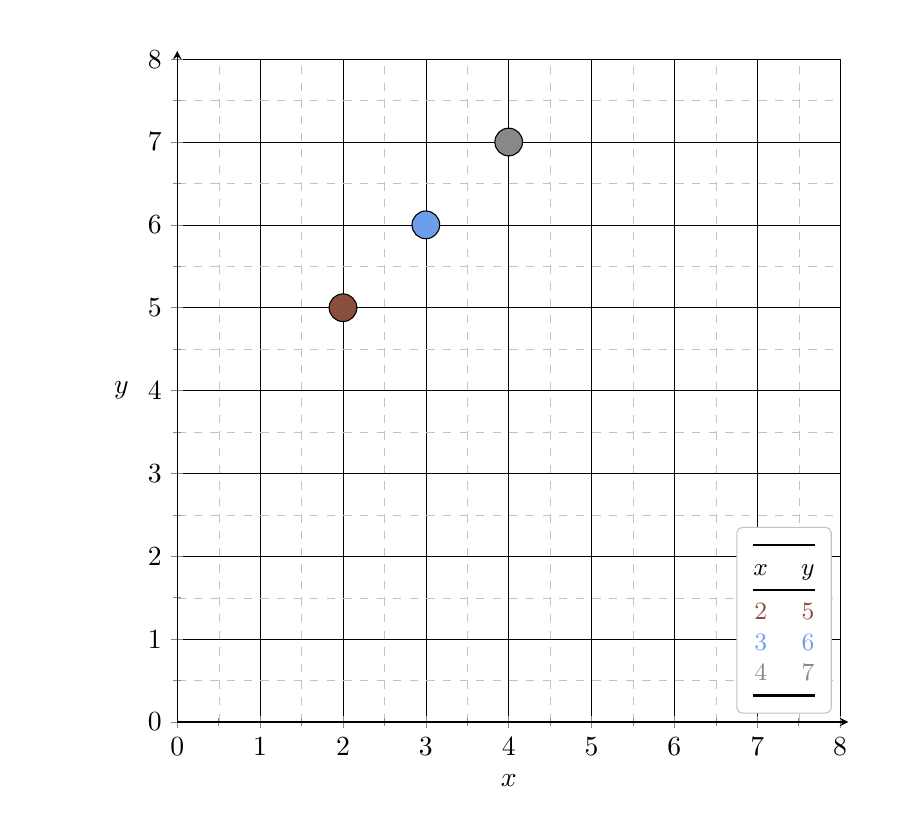
\begin{tikzpicture}
  \begin{axis}[
    set layers,
    axis lines=left,
    x axis line style={->,>=stealth, shorten >=-3pt},
    y axis line style={->,>=stealth, shorten >=-3pt},
    xlabel={\(x\)},
    ylabel={\(y\)},
    ylabel style={rotate=-90},
    xmin=0, xmax=8,
    ymin=0, ymax=8,
    xtick={0,1,...,8},
    ytick={0,1,...,8},
    axis equal,
    minor x tick num=1,
    minor y tick num=1,
    grid=both,
    major grid style={line width=0.2pt,draw=black},
    minor grid style={line width=0.1pt,draw=gray!50,dashed},
    width=10cm,
    height=10cm,
  ]
    % Data points
    \addplot[only marks, mark=*, mark options={scale=2.5, fill=brown}]
      coordinates {(2,5)};
    \addplot[only marks, mark=*, mark options={scale=2.5, fill=blue}]
      coordinates {(3,6)};
    \addplot[only marks, mark=*, mark options={scale=2.5, fill=gray}]
      coordinates {(4,7)};

    % Dataset table (on foreground layer, above grid)
    \begin{pgfonlayer}{axis foreground}
    \node[anchor=south east, fill=white, draw=gray!50,
          inner sep=6pt, rounded corners=2pt] at (axis cs:7.9,0.1) {%
      \small
      \begin{tabular}{@{}cc@{}}
        \toprule
        $x$ & $y$ \\
        \midrule
        \textcolor{brown}{2} & \textcolor{brown}{5} \\
        \textcolor{blue}{3} & \textcolor{blue}{6} \\
        \textcolor{gray}{4} & \textcolor{gray}{7} \\
        \bottomrule
      \end{tabular}%
    };
    \end{pgfonlayer}
  \end{axis}
  \pgfresetboundingbox
  \useasboundingbox ([xshift=-19mm, yshift=-11mm]current axis.south west)
    rectangle ([xshift=4mm, yshift=4mm]current axis.north east);
\end{tikzpicture}
\end{document}
